\chapter{Discussion}\label{ch:discussion}

\section{Answers to the research questions}
\begin{description}[leftmargin=2.6em,style=nextline]
\item[RQ1] \textbf{The meeting loss does not save compute} in this setting. In a pre-registered test on 20 paired seeds it needed about a third more FLOPs than a tuned baseline ($+36.9\%$ and $+35.5\%$) because it costs $23\%$ more per step and does not reduce the number of steps; a same-cost deep-supervision control was level with the baseline, and none of seven further variants and controls was cheaper (\cref{ch:study1}).
\item[RQ2] The measurements are consistent with a \textbf{redundancy} explanation: the signal is aligned with the task gradient (cosine $0.75$--$0.80$), lives on the same few high-loss rows, is small at its tuned weight, and no tested larger weight gave a gain of $10\%$ or more; in ReLU larger weights destabilise the middle state (\cref{ch:mechanism}). This is an interpretation: the checks that would separate ``redundant'' from ``bad target'' were not run.
\item[RQ3] \textbf{A selective backward pass saves FLOPs}: $35.1\%$ and $38.4\%$ against the tuned baseline and $30.2\%$ and $35.5\%$ against a tuned small-batch baseline, in every one of 20 seeds; a random subset of rows of the same size is worse than the full pass (\cref{ch:study2}). The saving in time per step measured on one CPU is much smaller than the saving in FLOPs.
\item[RQ4] \textbf{Keeping fewer rows and dropping the warm-up matter}, and the resulting variant S20w0 needed $48.5\%$ and $48.8\%$ fewer FLOPs than the baseline and $46.5\%$ and $53.6\%$ fewer than a tuned Selective-Backprop reimplementation. The latter advantage comes from not paying for extra selection passes (\cref{ch:study3}).
\item[RQ5] \textbf{Tuning on two seeds is unreliable}: two tunings of the same baseline tied at selection but differed by up to $34\%$ on fresh seeds, and which baseline is used can reverse the verdict about an arm (\cref{sec:noise}). \textbf{FLOPs and time disagree}, and step counts and FLOPs can rank methods in opposite orders (\cref{sec:metrics}).
\end{description}

\section{Why a single cost metric is not enough}\label{sec:metrics}
\Cref{fig:metrics} puts the central metric problem in one picture. In optimiser \emph{updates}, Selective-Backprop is the best of the methods ($0.64$ of the baseline's updates to $0.975$) and S20w0 is nearly level with the baseline ($0.92$). In counted \emph{FLOPs}, the order is reversed: S20w0 needs $0.51$ of the baseline's FLOPs, and the released Selective-Backprop $1.10$ ($0.95$ if the selection pass were reused). In \emph{time per step}, a FLOPs saving of $39\%$ for S30 becomes $18\%$ (one thread) or $9\%$ (eight threads). Each metric answers a different question, and the choice among them has to be made, and stated, before the comparison. This agrees with the general warning that cost indicators can contradict each other \citep{dehghani2022efficiency}. The report chose FLOPs because they are deterministic, hardware-independent and charge every extra pass, and reports the limitations of that choice.

\begin{figure}[t]
\centering
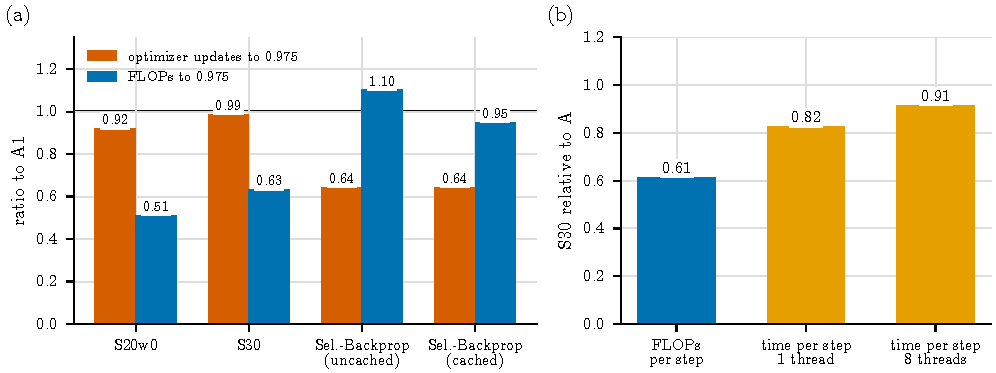
\includegraphics[width=\textwidth]{fig_metrics}
\caption{(a) The same runs ranked by two cost metrics (ratio to A1, target $0.975$, 20 seeds of Study 3). Optimiser updates favour Selective-Backprop; FLOPs favour S20w0. (b) For S30, the saving in time per step (one CPU, median of three repeats) is smaller than the saving in FLOPs per step.}
\label{fig:metrics}
\end{figure}

\section{Lessons on baselines and protocol}\label{sec:lessons}
\paragraph{The baseline is a distribution, not a number.} The six tunings of the same baseline, each tied to the others in design and budget, differ in mean cost by a factor of $1.34$ ($0.97$) and $1.18$ ($0.975$) on the Study~2 seeds, and $1.35$ and $1.16$ on the Study~3 seeds (\cref{tab:shift}). A comparison against one tuning therefore carries an uncertainty that is larger than the seed-to-seed variation. The protocol responded in two ways: it measured the shift between tunings and required the gain to exceed it, and it fixed the reference baseline in advance. The differences among the five re-tunings other than A2 are small and not stable: the sign of A6's change flips between the two seed sets at $0.97$, and that of A8 at $0.975$ (\cref{tab:shift}), which is what a selection of the minimum of a noisy score should be expected to produce.

\begin{table}[t]
\centering\small
\caption{Paired change (\%) of each re-tuning of the baseline against A1 on the same 20 seeds, in two independent seed sets, and the ratio of the largest to the smallest mean cost of the six tunings. A2 is much worse than the others in both sets.}
\label{tab:shift}
\begin{tabular}{@{}l rr rr@{}}
\toprule
 & \multicolumn{2}{c}{Study 2 seeds} & \multicolumn{2}{c}{Study 3 seeds}\\
\cmidrule(lr){2-3}\cmidrule(l){4-5}
Re-tuning & to 0.97 & to 0.975 & to 0.97 & to 0.975\\
\midrule
A2 & $+26.2$ & $+13.4$ & $+32.4$ & $+11.3$ \\
A5 & $-5.5$ & $-3.0$ & $-2.1$ & $-4.0$ \\
A6 & $-1.0$ & $-3.4$ & $+3.2$ & $-1.4$ \\
A7 & $-2.6$ & $-3.9$ & $-0.3$ & $-2.8$ \\
A8 & $+6.3$ & $+3.5$ & $+5.6$ & $-0.2$ \\
\midrule
max/min of the six means & 1.336 & 1.180 & 1.353 & 1.160
\\
\bottomrule
\end{tabular}
\end{table}

\paragraph{Selection scores are optimistic.} The winner of 25 trials on 2 seeds is the minimum of a noisy score, so its selection value is biased low, and it is an unreliable guide to its final value (\cref{fig:tuning-noise}). Arms that are tuned \emph{once} (B, D, SBT, S30T) have a different and unknown selection bias than the baseline, which was tuned six times and enters comparisons through A1 only. A cheaper remedy than more seeds in the search is to re-evaluate the best few trials on fresh seeds before choosing.

\paragraph{Pre-registration changes what can be claimed.} Because the decision rule included a definition of ``refuted'', the failure of the meeting loss could be stated as a result with an interval, and the failure of H6 ($B$ against $A$) could not be turned into a success by switching to the other tuning of the baseline. It also costs effort, and it does not remove every degree of freedom (\cref{app:deviations}): the rules were written by the same people who ran the experiments, and several choices (the crossing rule, the shift rule, the interval convention of Study~3) were made after earlier data were seen. What it changes is that these choices are visible and dated.

\paragraph{Exploration followed by a locked confirmation worked.} The two positive results were generated by exploratory looks, shrank slightly on new seeds (the winner's curse; \cref{sec:s3-explore}), and were then tested on fresh seeds with rules that could have returned ``refuted''. Both confirmatory effects were close to the exploratory estimates.

\section{Threats to validity and limitations}\label{sec:limitations}
\paragraph{Scope.} All results concern one 270\,000-parameter MLP on MNIST, with AdamW, batch size 128, a 3\,000-step horizon and one validation split. MNIST is easy, so accuracy targets of $0.97$ and $0.975$ are reached after about $7$ epochs at most; harder tasks may behave differently, and the hand-written selective backward pass only supports plain MLPs (no dropout, no batch normalisation). The report makes no statement about convolutional networks, transformers or GPUs. A reviewer at a machine-learning venue would regard a single small setting as insufficient; \cref{sec:future} lists the second setting that is needed first.

\paragraph{FLOPs are not time.} Elementwise operations, the top-$k$, the row gather and interpreter overhead are not counted. Time per step was measured only for S30 on one CPU with three repeats; S20w0 and Selective-Backprop were not timed; a derived estimate of time-to-target suggests the wall-clock gain of S30 might vanish at this model size. The headline numbers are therefore savings in counted FLOPs, and the claim that the method ``saves compute'' has to be read in that sense.

\paragraph{Selective-Backprop is a reimplementation.} It follows the released algorithm and code, in a small MLP, counting FLOPs. Its published gains are wall-clock gains on deep convolutional networks, where the backward pass dominates and a GPU is used. The report does not claim that S20w0 beats Selective-Backprop in general, only in this setting and under this counting. $\beta$, the history length and the priming length were fixed, not searched.

\paragraph{Conditional on tuned configurations.} Each arm's result depends on its tuned hyper-parameters (\cref{app:hyperparameters}). The selective arms inherit the baseline's configuration (S tuned once, in a descriptive group, gave no better result). The meeting loss, deep supervision and Selective-Backprop were tuned once each with 25 trials on two seeds, the baseline six times.

\paragraph{Metric and sampling.} The validation set has 5\,000 images, a single evaluation has a standard error of about $0.22$ percentage points at $0.975$, and a target is reached under a two-consecutive-evaluations rule defined after seeing noisy first crossings. The target $0.98$ was not usable as a primary target. All accuracy statements are about the validation split that was also used for tuning and for defining targets; the test set was not used, so the report makes no claim about test accuracy.

\paragraph{Researcher degrees of freedom and process.} Pre-registration here means locking hypotheses in a git repository, not an external registry, and the timestamps are those of git. The post-hoc and delegated decisions are listed in \cref{app:deviations}. The research process involved AI assistants that wrote code, analysis scripts and drafts of decisions, with the researcher accepting or changing them; the repository documents who decided what. This is a transparency fact and a possible source of undetected error, mitigated by reproducing the numbers from raw logs with independent scripts (\cref{app:reproducibility}).

\paragraph{Mechanisms are not established.} The redundancy explanation of the meeting-loss result rests on three small checks and was not tested by oracle or replacement arms. No mechanism is supported for the benefit of removing the warm-up.

\section{Relation to prior work}
The finding that selective backward passes save FLOPs in a small MLP is consistent with the motivation of Selective-Backprop \citep{jiang2019selective} and of Ordered SGD and online hard example mining \citep{kawaguchi2020ordered,shrivastava2016ohem}; it does not extend them. The finding that its advantage is partly an accounting matter (extra selection passes) is a caution when comparing methods that use different amounts of forward work. The warning of \citet{kaddour2023notrain} that apparent gains of efficient-training methods can vanish against a strong baseline is a reason to repeat the studies of this report with a fully decayed schedule in other settings; the baseline here is tuned, cosine-scheduled, and re-tuned six times, but only in one setting. The null result for the meeting loss agrees in spirit with the report that target-propagation methods do not scale \citep{bartunov2018assessing}, but it is a different claim: it concerns an auxiliary use, a compute metric and a small setting.

\section{Practical implications}
For a practitioner with a plain MLP and a compute budget measured in counted operations, the selective backward pass is a cheap thing to try: it needs a few lines of code, no extra network, and the evidence here is that keeping the highest-loss $20$--$30\%$ of each batch, with no full-backward warm-up, saves a large share of the FLOPs. Whether it saves \emph{time} on a given machine has to be measured on that machine. For a researcher evaluating a new training idea, the main practical points are: fix the baseline and the cost metric before looking; tune the baseline at least as much as the method and re-tune it to measure how much that matters; count every pass; use paired seeds; and write down what would make you say it failed.
